% XXX Jedes Jahr Professoren-Texte aktualisieren!
\section[Eure Profs stellen sich vor]{Eure Professoren stellen sich vor}
\textbf{Auf den folgenden zwei Seiten stellen sich eure beiden Professoren vor.
    Sie werden gemeinsam die "Physik~1" bis "Physik~3" lesen.
    Prof.\ Kulesza wird sich dabei um die theoretischen und Prof.\ Andronic um die experimentellen Aspekte des Studiums kümmern.
    Zudem stellt sich Prof.\ Werner vor, der die Vorlesungen "Mathematik für Physiker" halten wird (ebenfalls über drei Semester).
	Da diese drei Professoren euch eine Zeit lang begleiten werden, ist es durchaus mal interessant zu wissen, was sie gemacht haben, bevor sie an die Uni Münster kamen, und wie ihre aktuelle Forschung aussieht.}

\begin{multicols}{2}
\begin{center}
	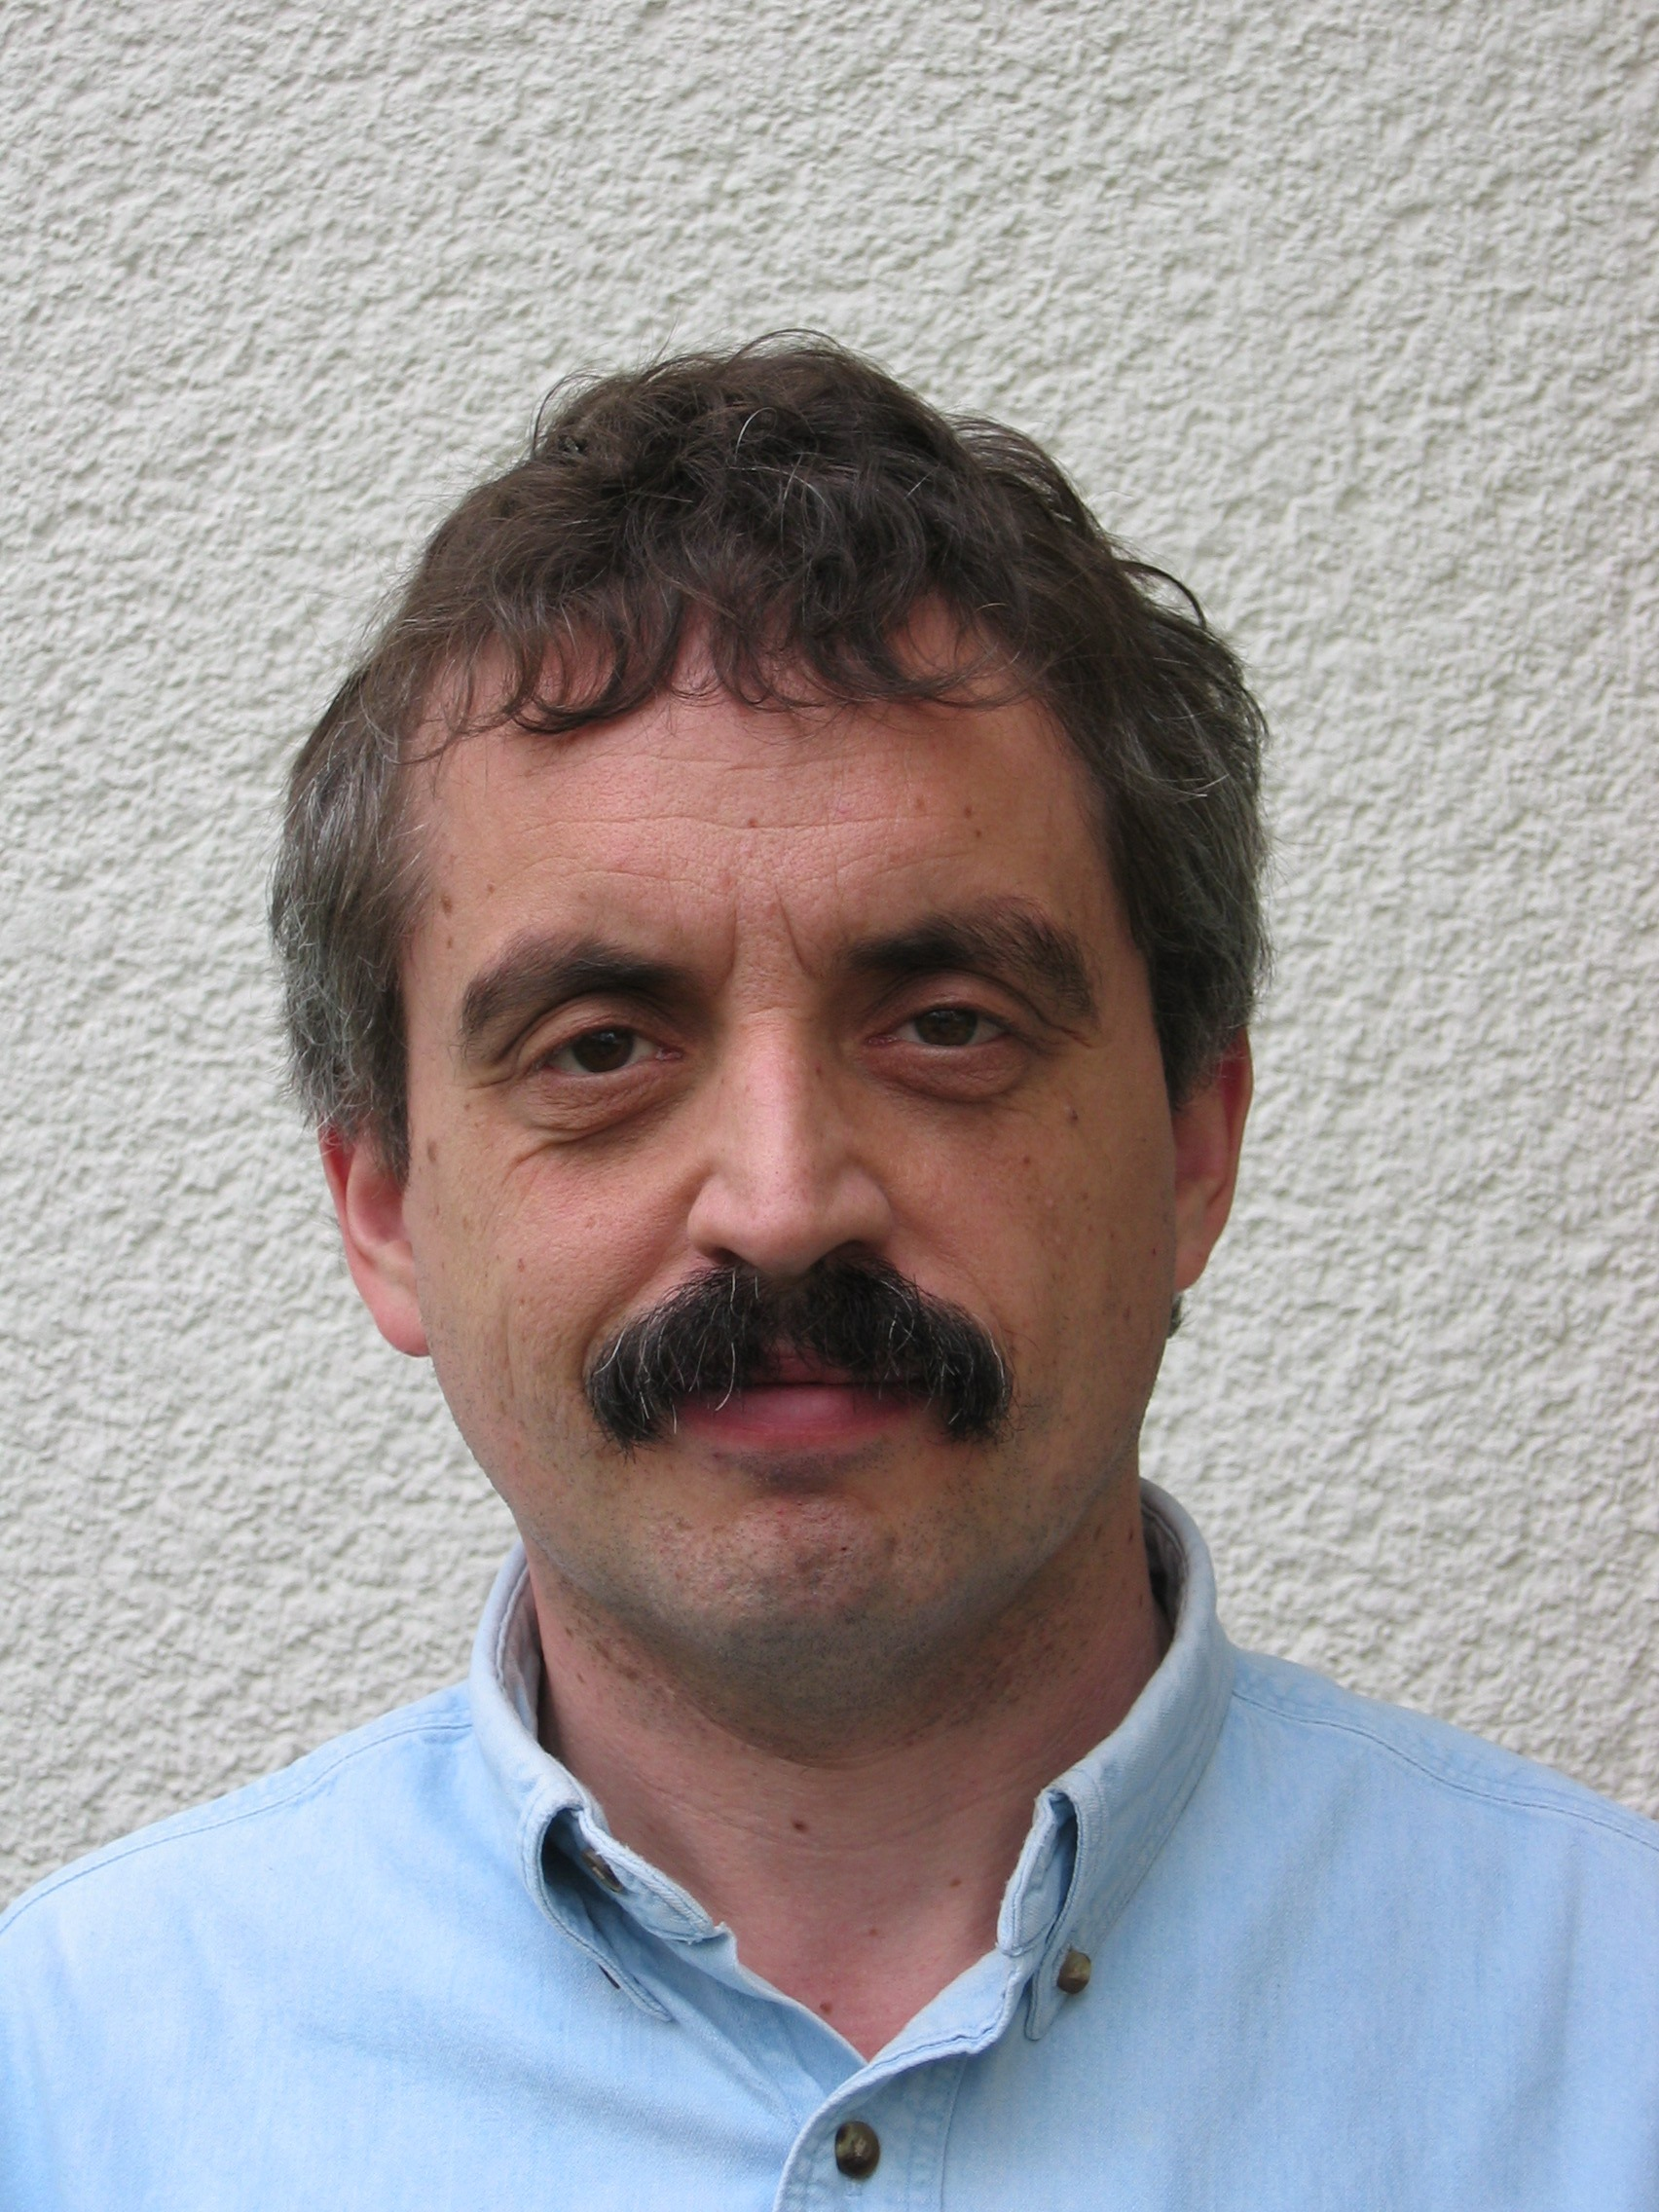
\includegraphics[width=\columnwidth, height=0.35\textheight]{res/vorstellungsfotos/wend_werner.jpg}\\
\smallskip
	Apl.\ Prof.\ Dr.\ Wend Werner\\
	Mathematisches Institut
\end{center}

Mir werden Sie in der nächsten Zeit in den Vorlesungen zur "Mathematik für Physiker" begegnen.
Mein Studium von Mathematik und Physik habe ich an der Freien Universität Berlin absolviert; Diplom und Promotion habe ich auch jeweils dort abgeschlossen.
Meine Habilitation habe ich an der Universität Paderborn gemacht und bin nun seit gut einem Jahrzehnt Hochschullehrer in Münster.

\[
	\resizebox{0.4\columnwidth}{!}{
		$\displaystyle\sum_{n = 1}^\infty \frac{1}{n^2} = \frac{\pi^2}{6}$
	}
\]

Die Themen von Promotion und Habilitation betrafen geometrische Fragen in Räumen unendlicher Dimension.
In letzter Zeit war das vor allem "Nichtkommutative Geometrie", ein Gebiet, welches versucht, einen mathematischen Formalismus zu finden, der in der Lage ist, Quanten- und relativistische Physik in einheitlicher Weise zu beschreiben.
Wie so oft beim Zusammenspiel von Mathematik und Physik sind auch hier interessante, rein mathematische Fragestellungen in Erscheinung getreten.

%\begin{center}
%	\includegraphics[width=\columnwidth, height=0.17\textheight]{private/res/comics/calvin_mathe.pdf}
%\end{center}

Der Zyklus "Mathematik für Physiker" ist eine kleine Herausforderung, da in vergleichsweise kurzer Zeit eine größere Stoffmenge vermittelt werden muss, die nichtsdestotrotz von den Teilnehmern anschließend handwerklich beherrscht werden muss.

Aber, keine Angst: Wir werden sehr langsam beginnen und erst im Laufe der Zeit Fahrt aufnehmen.
\end{multicols}

\begin{center}
	\fibelimgtext{
		\includegraphics[width=0.9\textwidth]{res/xkcd/435_purity.png}
	}{\url{https://xkcd.com/435}}
\end{center}

\newpage

\vspace*{\fill}

\begin{multicols}{2}
\begin{center}
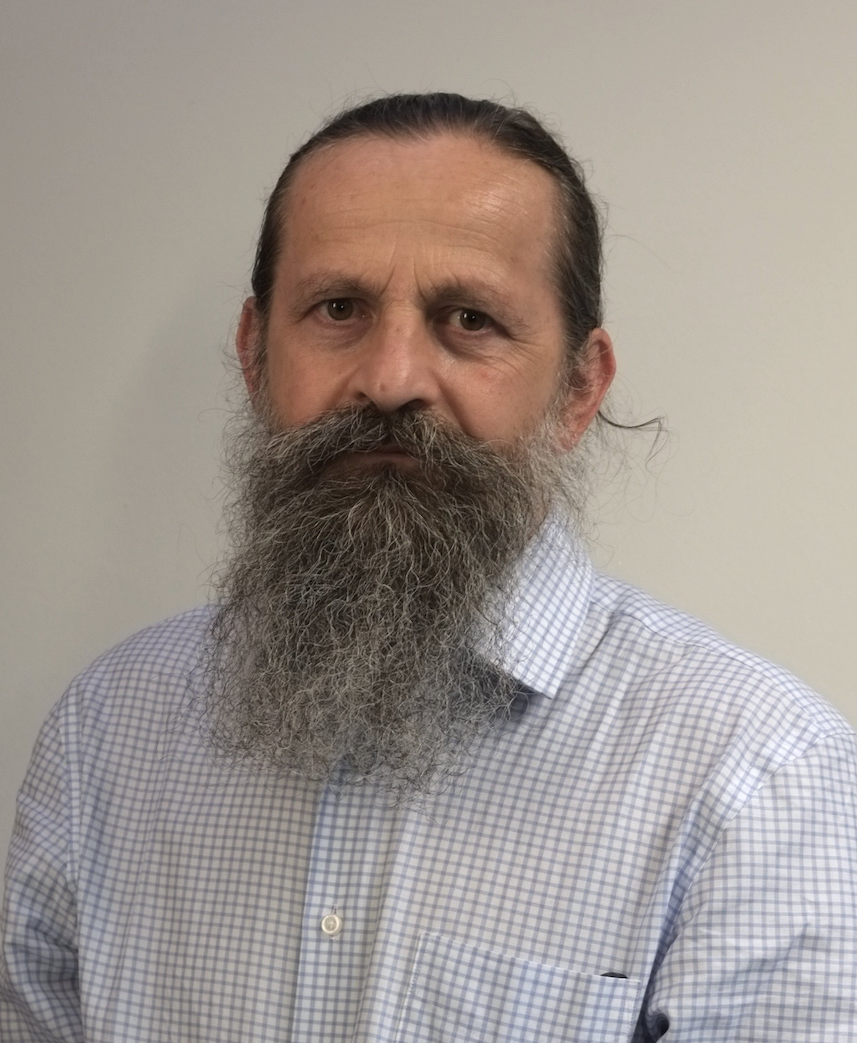
\includegraphics[width=0.8\columnwidth]{res/vorstellungsfotos/andronic.png}\\
\smallskip
Prof.\ Dr.\ Anton Andronic\\
Institut für Kernphysik
\end{center}

Ich freue mich sehr, mich gemeinsam mit Ihnen im Integrierten Kurs Physik 1-3 mit den Grundlagen der Physik zu befassen. Genauer liegt meine Verantwortung beim experimentellen Teil dieses Kurses.

Ich habe Physik an der Universität Bukarest studiert, wo ich in den kommunistischen Umbruchzeiten (1990) mein Diplom abgeschlossen habe. Nach ein paar Jahren als Junior-Wissenschaftler am Institut für Kernphysik in Bukarest habe ich meine Doktorarbeit über die kollektiven Eigenschaften der Kern-Kern Stösse mit dem Beschleuniger am Forschungsinstitut GSI in Darmstadt angefangen. Schon
während dieser Zeit habe ich mehrmals die GSI besucht, wo ich einen Teil meiner Arbeit, der nicht in Bukarest möglich war, durchführte. Ich habe 1998 in Bukarest promoviert und war sehr glücklich einen 1-Jahr-Vertrag als Postdoktorand an der GSI zu bekommen. Ich blieb doch mehrere Jahre, seit 2005 auf einer wissenschftlichen Mitarbeiter Stelle. Ich forschte für die Vorbereitung eines Experimentes (mit dem schönen Namen ALICE) am Large Hadron Collider am CERN in Genf. Mit den Teilchendetektoren, die ich entwickelte, haben ich und meine Kollegen Kollisionen am LHC erst im Jahr 2009 gemessen. Nach mehreren Jahren spannender Forschung mit ALICE am LHC habilitierte ich mich 2015 an der Technischen Universität Darmstadt. Seit 2018 bin ich Professor am Institut für Kernphysik der Westfälischen Wilhelms-Universität.

Ich erforsche die Eigenschaften eines extremen Zustands der Materie, der aus Quarks und Gluonen, den elementaren Bausteinen der starken Wechselwirkung (die auch die Eigenschaften der Atomkerne bestimmt) besteht. Solche Materie existierte im fruehen Universum bis etwa 10 Mikrosekunden nach dem Urknall und vermutlich existiert auch in den Kernen der Neutronensternen. Im Labor produzieren wir diese extrem dichte und heiße Materie in Kollisionen von Bleikernen am LHC. Die Ausdehnung ist sehr winzig und die Lebensdauer unglaublich kurz (10--23 Sekunden), trotzdem haben meine Kollegen und ich es geschafft, die Temperatur der Quark-Gluon-Materie zu bestimmen: diese Materie ist 100000 Mal so heiß wie im
Zentrum unserer Sonne (mit 10 Millionen Grad schon sehr heiß). Und, änlich wie (nahezu) im Urknall, besteht die am LHC produzierte Quark-Gluon-Materie nicht nur aus Materie: wir messen einen gleichen Anteil von Antimaterie.

Die Grundlagen der Kern- und Teilchenphysik werden Sie erst im 5. Semester lernen, auf dem Weg werden wir uns zusammen auf Mechanik, Thermodynamik, Elektrodynamik, etc. konzentrieren. Die Grundlagen in diesen Bereichen der Physik sind relevant für das Verständnis der Phänomene die leichter spürbar sind und werden Ihren auch ermöglichen, später selbst aktiv mitzuforschen. Ich hoffe, Ihre ersten Semester in Physik an der Uni werden interessant sein und auch Spaß machen!

\begin{center}
\includegraphics[width=0.7\columnwidth]{private/res/comics/manchmal_edited.jpg}\\
{\footnotesize 
S.~Harris – sciencecartoonsplus.com}
\end{center}

\end{multicols}

\vfill

\newpage

\vspace*{\fill}

\begin{multicols}{2}
\begin{center}
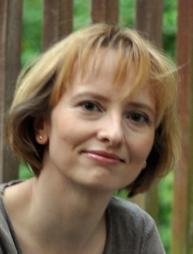
\includegraphics[width=0.71\columnwidth]{res/vorstellungsfotos/kulesza.jpeg}\\
\smallskip
Prof.\ Dr.\ Anna Kulesza\\
Institut für Theoretische Physik
\end{center}

In den nächsten drei Semestern werden wir uns gemeinsam in den Modulen Physik 1-3 mit den Grundlagen der Physik befassen. Im Rahmen des “integrierten Kurses” werden Herr Prof. Dr. Anton Andronic und ich experimentelle und theoretische Aspekte parallel vorstellen, wobei ich für den theoretischen Teil zuständig bin.

Seit dem Sommersemester 2012 bin ich Professorin am Institut für Theoretische Physik der Westfälischen Wilhelms-Universität Münster. Meine Forschungsinteressen liegen im Bereich der Teilchenphysik und deren Phänomenologie, die eine Brücke zwischen der Theorie und den Experimenten darstellt. In meiner Arbeitsgruppe untersuchen wir z.B. die Erzeugung von Higgs Bosonen oder Top Quarks am Large Hadron Collider (LHC) am CERN (Europäische Organisation für Kernforschung) in der Nähe von Genf in der Schweiz. Mit meiner Forschungsarbeit unterstütze ich auch die Suche am LHC nach hypothetischen Teilchen, die von verschieden neuen theoretischen Modellen vorhergesagt werden. 

Mein Weg in der Wissenschaft hat an der Universität Warschau angefangen. Schon vor Ende meines Physikstudiums bin ich nach England umgezogen, wo ich drei Jahre später an der Durham University promoviert habe. Nach meiner Promotion hat es mich noch weiter, nämlich in die USA, gezogen, wo ich dann drei Jahre am Brookhaven National Laboratory, einem Labor in der Nähe von New York forschte. Im Anschluss kehrte ich zurück nach Europa und war sowohl an den Universitäten in Karlsruhe und in Aachen als auch am Forschungslabor DESY in Hamburg als Wissenschaftlerin tätig. Seit ich an die WWU berufen wurde, leite ich die Arbeitsgruppe „Hadron collider phenomenology“. 

Trotz der COVID Pandemie hoffe ich, dass Sie Ihr Studium genießen können und natürlich viel Spaß an der Physik haben werden!

\end{multicols}

\vspace*{\fill}

\begin{center}
	\fibelimgtext{
		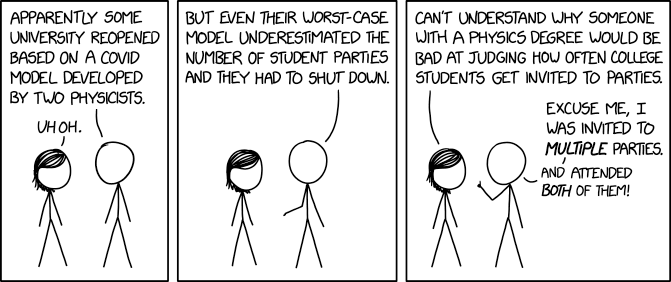
\includegraphics[width=0.9\textwidth]{res/xkcd/2355_university_covid_model.png}
	}{\url{https://xkcd.com/2355}}
\end{center}

\vfill
